\section{Matroid definiciója és a rangfüggvény szubmodularitása}

A matroidot definiálhatjuk a függetlenségi axiómákkal mint, legyen $E$ egy
tetszőleges és véges alaphalmaz. Ugyanakkor $F \subseteq  2^E$ egy halmaz
rendszer. Egy adott $M=(E,F)$ struktúra matroid, ha teljesül, hogy:

\[
\begin{cases}
\mbox{F1}) &\emptyset \in F \\
\mbox{F2}) &\begin{rcases}
X \in F \\ 
Y \subseteq X 
\end{rcases} \Rightarrow \parbox[L]{11cm}{$Y \in F$
($F$ \emph{leszálló halmazrendszer} -- ha egy halmaz benne van $F$--ben akkor annak összes
részhalmaza is benne van $F$--ben, ehhez szükséges az F$1$ axióma).
} \\
\mbox{F3}) &\begin{rcases}
X,Y \in F\\
|X| > |Y| \\
\end{rcases} \Rightarrow\parbox[t]{10.5cm}{ $\exists~x \in X-Y$,~hogy $Y \cup \{x\}
\in F~($\emph{szubmodularitás, kölcsönösen bővithetőség} -- legyen két halmazrendszer
a matroidból, ahol ez egyik számoságban több elemet tartalmaz; ha e több
eleműben létezik olyan elem amely a kisebbikben nincs, akkor ezzel a kisebbiket
kiegésztive szintén $F$--beli elemet kapunk).}
\end{cases}
\]

Egy $M=(E,F)$ matroidban: 

\begin{description}
  \item[független halamaznak] nevezzük $E$ alaphalmaz $F$--hez tartozó
  részhalmazait ( tehát $X\subseteq E$--re $X \in F$).
  \item[maximális független halmaznak] nevezzük azt az $X \in F$ halmazt
  amelyhez már nem bővithető tovább anélkül, hogy a halmaz függetlensége
  sérüljön.
  \item[matroid bázisai] a matroid maximális független halmaza.
  \item[minimálisan összefüggő halmaznak] nevezzük azt az $X \ in F$ halmazt
  amely nem független, de amelyből bárhogy veszünk el egy elemet a művelet
  függetlené tesszi.
  \item[körnek] nevezzük a minimálisan összefüggő halmazt.
  \item[hurok] az egyelemű kör. 
  \item[a halmaz rangja] egy $X\subseteq E$ halmaznak az $X$ maximális
  független részhalmazának mérete, elemszáma. Jelölése: $r(X)$.
  \item[a matroid rangja] az alaphalmaz rangja, azaz $r(E)$, ahol $r:2^E \mapsto \mathbb{Z}^+$.
\end{description}

\emph{Legyen $M=(E,F)$ matroid ahol $A\subseteq E$ és $X_1,X_2 \in A$ maximális
független halmazok $A$--ban (bázisok), akkor $|X_1|=|X_2|$}. A bizonyitás
indirket megy, legyen $|X_1| > |X_2| \Rightarrow \exists e \in X_1-X_2$, ahol
F$3$ miatt $X_1\cup \{e\} \in F \Rightarrow X_1$ nem maximális. De ez
ellentmondás, tehát a feltevéssünk is hamis volt.

\begin{table}[htbp]
\begin{center}
\caption{Példák matroidra}
\begin{tabular}{>{\centering\arraybackslash}m{7cm}>{\centering\arraybackslash}m{4cm}>{\centering\arraybackslash}m{1.5cm}}
Lineáris (mátrix) matroid & Grafikus matroid & Uniform matroid \\ \hline
$
\left( \begin{array}{ccc}
\overbrace{1}^a & \overbrace{2}^b  \\
0 & 0
\end{array} \right)
$ &
\centering
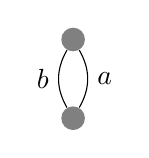
\begin{tikzpicture}[scale=1]
  \tikzset{ p/.style={circle,white,fill=gray,inner sep=0pt,minimum size=0.3cm},
  }
  \node[p] (1) at (0, 0) {};
  \node[p] (2) at (0, -1) {}; 
  
  % the connection between the dots
  \draw[bend left,-]  (1) to node [midway, right] {$a$} (2); 
  \draw[bend right,-]  (1) to node [midway, left] {$b$} (2);
\end{tikzpicture}
& $U_{2,1}$ \\ \hline
$
\left( \begin{array}{ccc}
\overbrace{1}^a & \overbrace{0}^b & \overbrace{1}^c  \\
0 & 1 & 1
\end{array} \right)
$ &
\centering
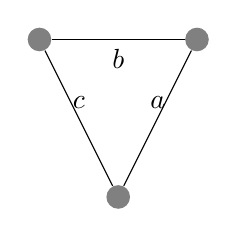
\begin{tikzpicture}[scale=1]
  \tikzset{ p/.style={circle,white,fill=gray,inner sep=0pt,minimum size=0.3cm},
  }
  \node[p] (1) at (0, -3) {};
  \node[p] (2) at (-1, -1) {}; 
  \node[p] (3) at (+1 , -1) {};
  
  % the connection between the dots
  \draw[-] (1) -- (2) node [midway, above] {$c$}; 
  \draw[-] (2) -- (3) node [midway, below] {$b$}; 
  \draw[-] (3) -- (1) node [midway, above] {$a$};
\end{tikzpicture}
& $U_{3,2}$ \\ \hline
$ \left( \begin{array}{ccccc}
\overbrace{1}^a & \overbrace{0}^b & \overbrace{1}^c & \overbrace{2}^d& \overbrace{0}^e  \\
0 & 1 & 1 &0&0
\end{array}  \right)
$
&
\centering
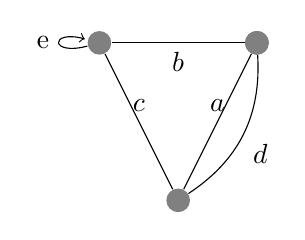
\begin{tikzpicture}[scale=1]
  \tikzset{ p/.style={circle,white,fill=gray,inner sep=0pt,minimum size=0.3cm},
  }
  \node[p] (1) at (0, -3) {};
  \node[p] (2) at (-1, -1) {}; 
  \node[p] (3) at (+1 , -1) {};
  \node[p] (4) at (+1 , -1) {};
  \node[p] (5) at (+1 , -1) {};
  
  % the connection between the dots
  \draw[-] (1) -- (2) node [midway, above] {$c$}; 
  \draw[-] (2) -- (3) node [midway, below] {$b$}; 
  \draw[-] (3) -- (1) node [midway, above] {$a$};
  \draw[bend left,-]  (3) to node [auto] {$d$} (1);
   \path (2) edge[loop left] node[left] {e} (2);
\end{tikzpicture}
& $|E|=5,$ $32$ részhalmaz\\ \hline
$ \left( \begin{array}{ccccc}
\overbrace{1}^a & \overbrace{0}^b & \overbrace{1}^c & \overbrace{1}^d\\
0 & 1 & 1 &2
\end{array}  \right)
$
& $\not \exists$
& $U_{4,2}$\\

\end{tabular}
\end{center}
\end{table}
 \begin{description}
  \item[Grafikus matroid] egy $G$ gráf által leírt $M=(G$ élei, $G$ --beli erdők). A bázis fogalma
  megfelel a feszítő erdőnek. Jelőlése $M(G)$ és még körmatroidnak is nevezzük.
  \item[Lineáris matroid] egy mátrix által indukált matroid $M=(A$ oszlopai, $A$ lineárisan
  független oszlopai). Mátrixmatroid név alatt is ismeretes.
  \item[Uniform matroid] egy $M=($ tetszőleges véges halmaz, a halmaz lefeljebb
  $k$ elemű részhalmazai). Legyen $n=|E|$. Ekkor $U_{n,k}$--val jelöljük az
  uniform matroidot. $U_{n,n}$ a teljes/szabad matroid (grafikusan egy csillag
  alakzat), ha összes részhalmaza független. $U_{n,0}$ a triviális matroid,
  amelyben csak az üres halmaz független (grafikusan minden éle egy hurok).
\end{description}

\subsection{Rangfüggvény szubmodularitása}
Bármely $X, Y \subseteq E$--re igaz, ha $r:2^E \mapsto \mathbb{Z}^+$ egy matroid
rangfüggvénye, akkor:

\[
\begin{cases}
\mbox{R1)}& r(\emptyset) = 0 \\
\mbox{R2)}& r(X) \leq |X| \\
\mbox{R3)}& r(Y) \leq r(X), \mbox{ ha } Y \subseteq X \\
\mbox{R4)}& r(X)+ r(Y) \geq r(X \cup Y) + r (X \cap Y)
\end{cases}
\]

Azaz (fordítva), ha $r$ egy egészérrtékű függvény $E$ részhalmazain, amelyre
teljesül a fenti négy tulajdonság, akkor $r$ egy $M=(E,F)$ matroid rangfüggvénye,
ahol:
\[F=\left\{ H : r(H)=|H| \right\}. \]

Az első három tulajdonság bizonyitása rögtön adódik a rang definiciójából. Az
R$4$--re meg (ami a rangfüggvény szubmodularitása) legyen egy $X,Y \in E$. $A$
egy maximálisan független halmaz $X \cap Y$--ban ($A \subseteq X \cap Y),$ amely
számossága $\alpha$. 

Nyilván $A$ kiterjeszthető egy B halmazzá úgy, hogy az maximálisan független
legyen $X \cup Y$--ban. Ehhez $X$--ből $\beta$ új elemet rakunk hozzá, és
$Y$--ból $\gamma$ darabot:
\begin{align*}
r(X \cap Y) &= \alpha \\
r(X \cup Y) &= \alpha + \beta + \gamma
\end{align*}

E számok korlátot szabnak $X$ és $Y$ rangjára is mint: 
\begin{align*}
r(X) &\geq \alpha + \beta \\ 
r(Y) &\geq \alpha + \gamma \\
r(X) + r(Y) &\geq \underbrace{\alpha + \beta + \gamma}_{r(X \cup Y)} + \underbrace{\alpha}_{r(X \cap Y)} \\
r(X) + r(Y) &\geq r(X \cup Y) + r(X \cap Y) \\
\end{align*}

\begin{figure}[htbp]
\centering
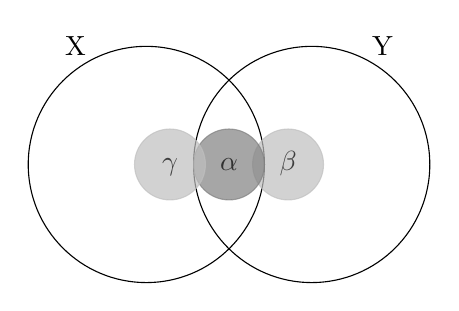
\begin{tikzpicture}[scale=3]
	\draw (0,0) circle (5mm)  (-3mm,5mm) node{X};
	\draw (7mm,0) circle (5mm)  (10mm,5mm) node[black]{Y};
	\begin{scope}[opacity=0.7]
    \filldraw[fill=lightgray, draw=lightgray] (6mm,0) circle (1.5mm) node[black, anchor=mid]{$\beta$};
 	\filldraw[fill=gray, draw=gray]  (3.5mm,0) circle (1.5mm) node[black,anchor=mid]{$\alpha$};
 	\filldraw[fill=lightgray, draw=lightgray]  (1.0mm,0) circle (1.5mm) node[black,anchor=mid]{$\gamma$};
	\end{scope}
\end{tikzpicture}
\caption{A rangfüggvény szubmodularitása}\label{fig:RangSzub}
\end{figure}

Példa arra, hogy az egyenlőség nem mindig áll fent:
\vspace{0.4cm}

\begin{tabular}{>{\centering\arraybackslash}m{3cm}>{\centering\arraybackslash}m{6cm}}
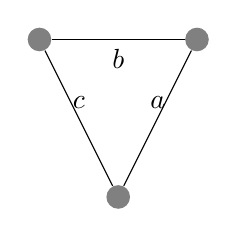
\begin{tikzpicture}[scale=1]
  \tikzset{ p/.style={circle,white,fill=gray,inner sep=0pt,minimum size=0.3cm},
  }
  \node[p] (1) at (0, -3) {};
  \node[p] (2) at (-1, -1) {}; 
  \node[p] (3) at (+1 , -1) {};
  
  % the connection between the dots
  \draw[-] (1) -- (2) node [midway, above] {$c$}; 
  \draw[-] (2) -- (3) node [midway, below] {$b$}; 
  \draw[-] (3) -- (1) node [midway, above] {$a$};
\end{tikzpicture} 
& $
\begin{cases}
X=(a,b), &r(X)=2 \\ 
Y=(a,c) &r(Y)=2  \\
X \cup Y, &r(X \cup Y)=2 \\
X \cap Y, &r(X \cap Y) = 1
\end{cases}
$ \\
\end{tabular}
